
\documentclass{../concepts/prepareprotokol} %všechny balíčky pro protokol + titulní strana
\usepackage{graphicx}
\usepackage{booktabs}
\usepackage{amsmath}
\usepackage{siunitx}
\sisetup{inter-unit-product =$\cdot$}
\sisetup{separate-uncertainty=true}

\praktikum{II} %číslo praktika (I, II nebo III)
\autor{David Němec} %jméno autora
\datum{DEN\,MĚSÍC\,2025} %datum měření
\cislo{ČÍSLO} %číslo úlohy
\nazev{NÁZEV} %název úlohy

\begin{document}
\maketitle

% ========================== PRACOVNÍ ÚKOL =========================
\section{Pracovní úkol}
\begin{enumerate}
    \item
\end{enumerate}

% ============================= TEORIE ===============================
\section{Teorie}
\subsection{Kapacita deskového kondenzátoru}


\subsection{Experimentální uspořádání}

\begin{figure}[htbp]
    \centering
    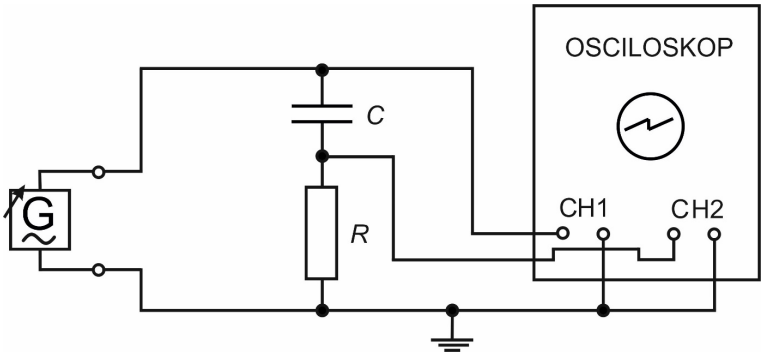
\includegraphics[width=0.5\linewidth]{uloha27/schema.png}
    \caption{Schéma zapojení [LITERATURA]}
    \label{fig:schema}
\end{figure}



\subsection{Měřicí přístroje a jejich nejistoty}
\begin{enumerate}
    \item PŘÍSTROJ:
    
    POZNÁMKY

\end{enumerate}
%\def\figurename{Obr\’azek}%
\def\figurename{Graf}%
\setcounter{figure}{0}

% ======================== VÝSLEDKY MĚŘENÍ ===========================
\section{Výsledky měření}


\begin{figure}
    \centering
    \includegraphics[width=0.5\linewidth]{uloha27/GRAF1.png}
    \caption{Závislost kapacity deskového kondenzátoru na napětí.}
    \label{fig:osciloskop}
\end{figure}


% ============================ DISKUZE ===============================
\section{Diskuze}


% ============================= ZÁVĚR ================================
\section{Závěr}


% =========================== LITERATURA =============================
\section*{Literatura}
\begin{itemize}
\item 

[1] Kolektiv ZFP KVOF MFF UK: Měření dielektrických vlastností materiálů [online]. [cit. 26.10.2025], dostupné z https://physics.mff.cuni.cz/vyuka/zfp/\_media/zadani/texty/txt\_227.pdf

\item 

[2] Kolektiv ZFP KVOF MFF UK: Měření odporu [online]. [cit. 26.10.2025], dostupné \\
z https://physics.mff.cuni.cz/vyuka/zfp/\_media/zadani/texty/txt\_202.pdf

\item

[3] Kolektiv ZFP KVOF MFF UK: Měření dielektrických vlastností materiálů - pokyny k měření [online]. [cit. 26.10.2025], dostupné z https://physics.mff.cuni.cz/vyuka/zfp/\_media/zadani/pokyny/mereni\_227.pdf

\item 

[4] Kolektiv ZFP KVOF MFF UK: Měření dielektrických vlastností materiálů - fotodokumentace [online]. [cit. 26.10.2025], dostupné z https://physics.mff.cuni.cz/vyuka/zfp/\_media/zadani/foto/foto\_227.pdf

\item 

[5] J. Englich: Úvod do praktické fyziky I: Zpracování výsledků měření. 1. vyd. Praha: Matfyzpress, 2006

\item 

[6] Eite Tiesinga, Peter J. Mohr, David B. Newell, and Barry N. Taylor: Values of fundamental physics constants: Vacuum electric permittivity [online]. [cit. 27.10.2025], dostupné z https://physics.nist.gov/cgi-bin/cuu/Value?ep0

\item 

[7] Dinel s.r.o.: tabulka relativních permitivit [online]. [cit. 27.10.2025], dostupné z https://www.dinel.cz/ \\ \_file/AMIfv95QsvMopq8GA848o69r\_yFAVYgklqLiAoLME0ORLQPdCAIkRAeJvDDR90OQh8kq6T4bVT6 \\ 
dASBZ27h\_lIuHiZ3j-GhH8T6DphAz1Ui4CwS-441Bupe\_IVYYHw\_XkUqAHRt6U93WEiawC8m6jG7tzF1pt \\
cn0sQ/relativni-permitivity-cz\_n1.pdf

\item 

[8] Mikulčák a kolektiv: Matematické, fyzikální a chemické tabulky pro střední školy: relativní permitivita, Praha: Státní pedagogické nakladatelství, n. p., 1988

\end{itemize}
\end{document}